% !TEX root = main.tex

本课程采用书目Alfred V. Aho, Monica S. Lam, Ravi Sethi, Jeffrey D. Ullman, \emph{Compilers: Principles, Techniques \& Tools (2nd ed)},即大名鼎鼎的龙书。
同时也参考了\href{http://web.stanford.edu/class/cs143/}{Stanford CS143: Compilers}这门课程。

\section{简介}
编译器的几个阶段如下,前端包括词法(lexical)、语法(syntax)、语义(semantic)分析,中端IR生成、优化,后端代码生成。
\begin{figure}[H]
\centering
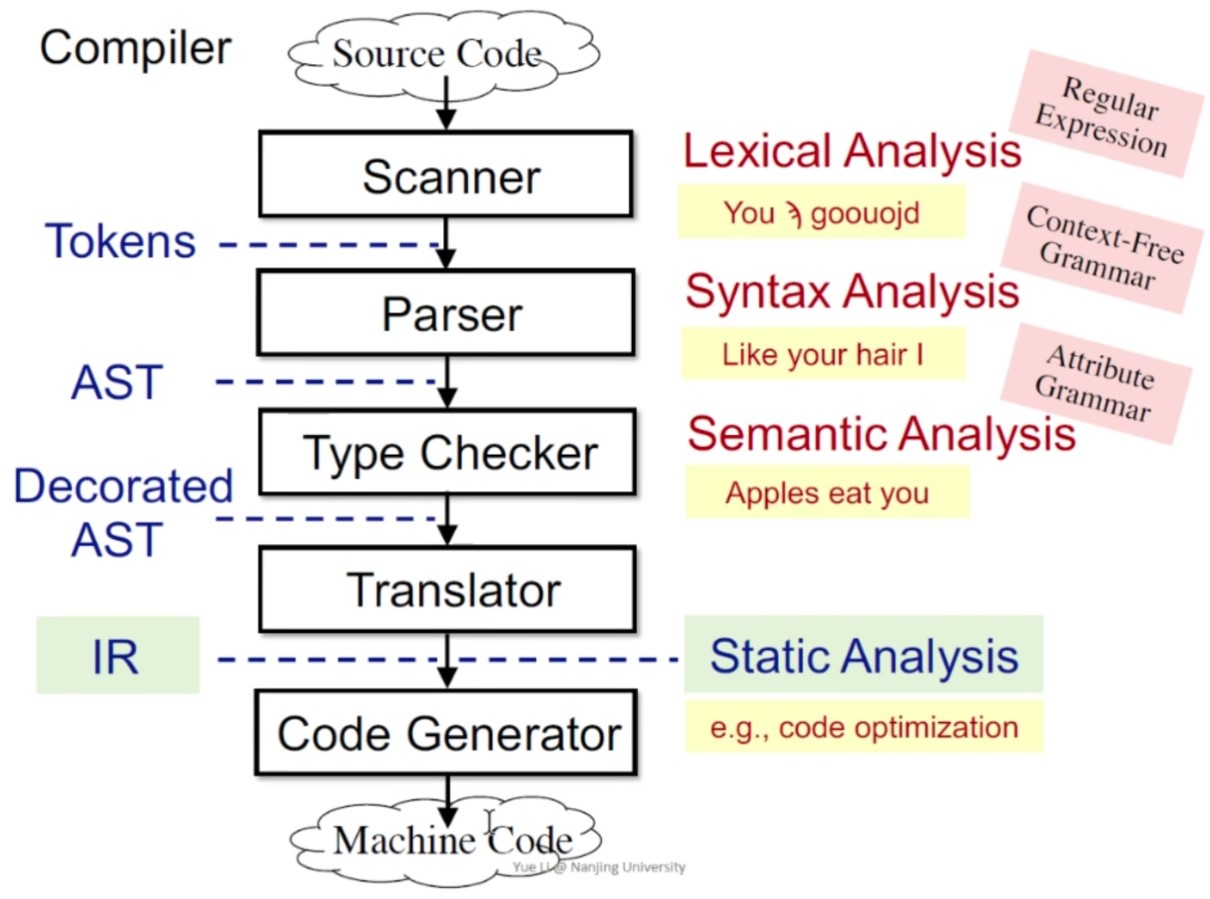
\includegraphics[width=0.6\linewidth]{fig/compiler_flow.jpg}
\end{figure}

编程语言设计的思想:
\begin{itemize}
	\item 抽象(abstraction):核心在于信息隐藏(infomation hiding),只把必要的暴露出来
	\item 类型(types):表达抽象、查出常见错误、使程序安全
	\item 重用(reuse):开发软件系统中常见的模式(类型参数化、类与继承)
\end{itemize}